%!TEX root = TDT4265-Summary.tex
\section{Epipolar geometry}
With one camera, you know the direction to each pixel/object in an image, but not its distance. With two cameras and epipolar geometry, this can be determined.

\begin{figure}[htbp]
    \centering
    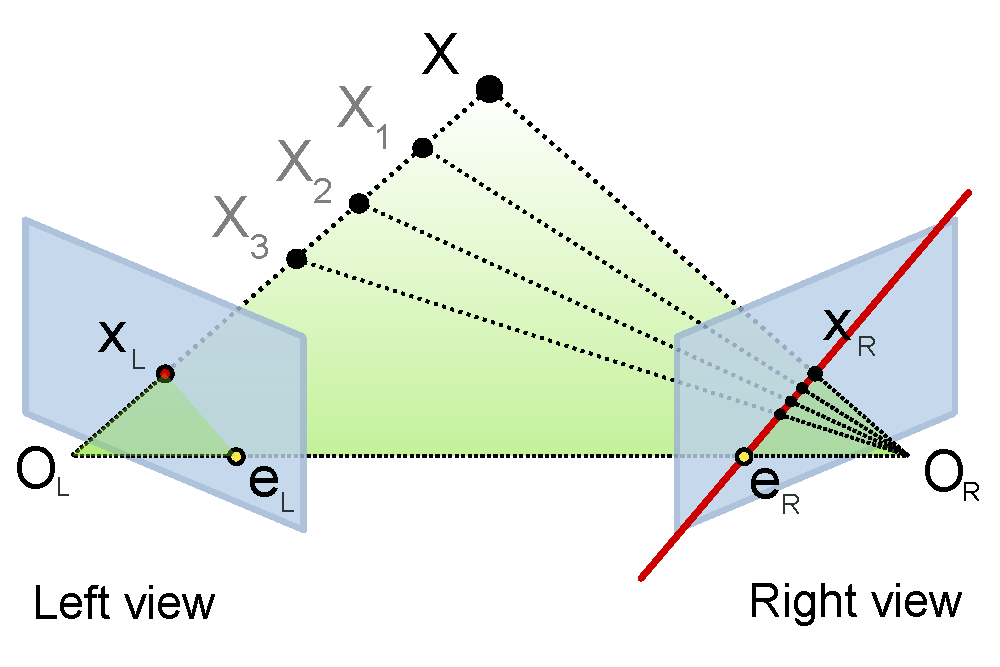
\includegraphics[width=0.95\linewidth]{images/Epipolar_geometry}
    \caption{Epipolar geometry}
    \label{fig:epipolar-geometry}
\end{figure}

In Figure \ref{fig:epipolar-geometry}, both cameras see the object $\V{X}$. The line $\V{O}_L$--$\V{X}$ from the left camera to $\V{X}$, is seen as the epipolar line $\e_R$--$\x_R$ by the right camera, marked in red. (Correspondingly, $\x_L$--$\e_L$ is an epipolar line for the left camera.) This means that $\V{X}$ must lie on the red epipolar line, but we don't know where (this is the fundamental ambiguity). This provides a constraint that can be used to create a model describing the geometric transformation between the two image planes.

\subsection{Essential matrix}
The epipolar constraint from the previous section can be formulated as
\begin{equation}
    \y_1\T \M{E} \y_0 = 0
\end{equation}
where $\y_1$ and $\y_0$ are normalized image coordinates and $\M{E}$ is the essential matrix. This relation holds if the coordinates correspond to the same point in 3D space. Thus, the essential matrix relates points in global coordinates.

\subsection{Fundamental matrix}
The fundamental matrix $\M{F}$ does the same as the essential matrix, but relates points given in image pixel coordinates, such as $\x_L$ and $\x_R$ in Figure \ref{fig:epipolar-geometry}. A similar relation holds for image coordinates that describe the same point in space:
\begin{equation}
    \x_1\T \M{F} \x_0 = 0
\end{equation}

\subsection{Structure from motion (SfM)}
SfM is a method for using data from many 2D images to create a 3D map. It's based on finding features in all the images taken (a huge amount is necessary). Match features between images to estimate camera location, and then pixel distances.
